% Intended LaTeX compiler: xelatex
\documentclass[10pt, svgnames]{beamer}
\usepackage{graphicx}
\usepackage{longtable}
\usepackage{wrapfig}
\usepackage{rotating}
\usepackage[normalem]{ulem}
\usepackage{amsmath}
\usepackage{amssymb}
\usepackage{capt-of}
\usepackage{hyperref}
\usetheme{focus}
\author{Sappinandana Akamphon}
\date{\today}
\title{Analysis of Axially Loaded Members}
\subtitle{ME 210: Mechanics of Materials}
\usepackage{booktabs}
\institute{Department of Mechanical Engineering, TSE}
\date{}
\usetikzlibrary{patterns,shapes}
\AtBeginSection[]{\begin{frame}{Outline}\tableofcontents[currentsection]\end{frame}}
\hypersetup{
 pdfauthor={Sappinandana Akamphon},
 pdftitle={Analysis of Axially Loaded Members},
 pdfkeywords={},
 pdfsubject={},
 pdfcreator={Emacs 30.0.50 (Org mode 9.6)}, 
 pdflang={English}}
\usepackage{biblatex}

\begin{document}


\begin{frame}[label={sec:org4ad1011}]{\{\}}
\maketitle
\end{frame}

\section{Overview of Axially Loaded Member Problems}
\label{overview-of-axially-loaded-member-problems}
\begin{frame}[label={sec:org9403e2e}]{Axially Loaded Member}
\begin{itemize}
\item Back to the basic: 1D stress-strain relationship

\item Load is applied along the axis

\item Load passes through the centroid

\item For now, ignore lateral deformation
\end{itemize}
\end{frame}

\begin{frame}[label={sec:orgfde4a5f}]{2 Types of Problems in Statics}
\begin{itemize}
\item Statically determinate: equilibrium equation is all you need

\item Statically Indeterminate Problems

\begin{itemize}
\item equilibrium isn't enough
\end{itemize}
\end{itemize}
\end{frame}

\section{Statically Determinate Problems}
\label{statically-determinate-problems}
\begin{frame}[label={sec:org0486a0e}]{Statically Determinate Axially Loaded Members}
\begin{itemize}
\item Simplest of them all

\item Well, simplest doesn't really mean simple

\item All you need is equilibrium equation\ldots{} and a smart way to use it
\end{itemize}
\end{frame}

\begin{frame}[label={sec:org66e4581}]{Elastic Deformation of Axially Loaded Members}
\begin{figure}[h]
  \centering
  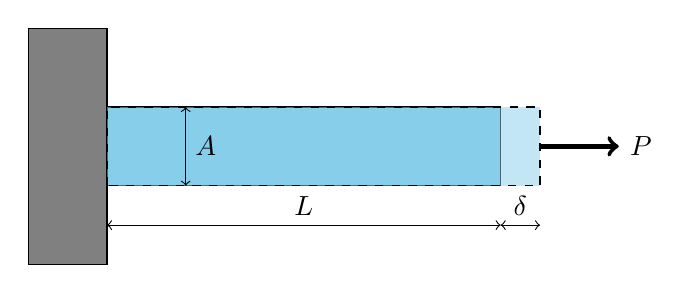
\begin{tikzpicture}
    \draw[fill=Grey] (-1,-1) rectangle (0,2);
    \draw[fill=SkyBlue] (0,0) rectangle (5,1);
    \draw[fill=SkyBlue, fill opacity=0.5, dashed] (0,0) rectangle (5.5,1);
    \draw[->,ultra thick] (5.5,0.5) -- (6.5,0.5) node[right]{$P$};
    \draw[<->] (0,-0.5) -- (2.5,-0.5) node[above]{$L$} -- (5,-0.5);
    \draw[<->] (5,-0.5)-- (5.25,-0.5) node[above]{$\delta$} -- (5.5,-0.5);
    \draw[<->] (1,0) -- (1, 0.5) node[right]{$A$} -- (1,1);
  \end{tikzpicture}
\end{figure}

\begin{itemize}
\item For any member with constant cross section

\begin{align*}
  \sigma(x) = \frac{P}{A} \varepsilon(x) = \frac{\delta}{L}
\end{align*}
\end{itemize}
\end{frame}

\begin{frame}[label={sec:orgbfb11bd}]{Hooke's Law}
\begin{align*}
  \sigma(x) &= E \varepsilon \\
  \frac{P}{A} &= E \frac{\delta}{L} \\
  \delta &= \frac{PL}{EA}
\end{align*}
\end{frame}

\begin{frame}[label={sec:orgd582fd4}]{Generalized Elastic Deformation}
\begin{figure}[h]
  \centering
  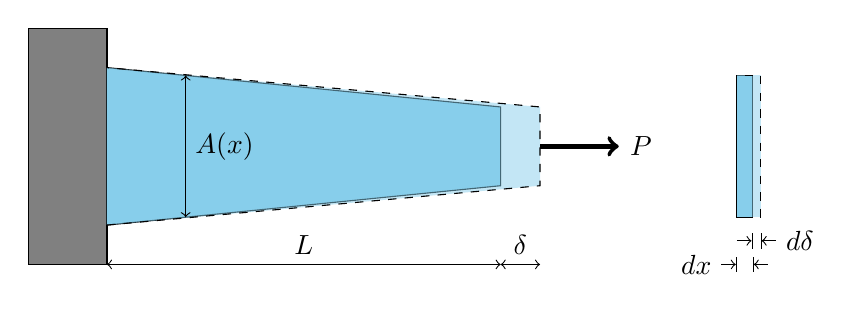
\begin{tikzpicture}
    \draw[fill=Grey] (-1,-1) rectangle (0,2);
    \draw[fill=SkyBlue] (0,-0.5) -- (5,0) -- (5,1) -- (0,1.5);
    \draw[fill=SkyBlue, fill opacity=0.5, dashed] (0,-0.5) -- (5.5,0) -- (5.5,1) -- (0,1.5);
    \draw[->,ultra thick] (5.5,0.5) -- (6.5,0.5) node[right]{$P$};
    \draw[<->] (0,-1) -- (2.5,-1) node[above]{$L$} -- (5,-1);
    \draw[<->] (5,-1)-- (5.25,-1) node[above]{$\delta$} -- (5.5,-1);
    \draw[<->] (1,-0.4) -- (1, 0.5) node[right]{$A(x)$} -- (1,1.4);

    \draw[fill=SkyBlue] (8,-0.4) rectangle (8.2,1.4);
    \draw[fill=SkyBlue, fill opacity=0.5, dashed] (8,-0.4) rectangle (8.3,1.4);
    \draw[->|] (7.8,-1) node[left]{$dx$}  to (8,-1);
    \draw[|<-] (8.2,-1) to (8.4,-1);
    \draw[->|] (8,-0.7) to (8.2,-0.7);
    \draw[|<-] (8.3,-0.7) to (8.5,-0.7) node[right]{$d\delta$};
  \end{tikzpicture}
\end{figure}
\normalcolor

\begin{align*}
  \sigma(x) &= E(x) \varepsilon(x) \\
  \frac{P(x)}{A(x)} &= E(x) \frac{d \delta}{dx} \\
  \delta = \int_0^L d \delta &= \int_0^L \frac{P(x)}{A(x)E(x)} dx
\end{align*}
\end{frame}

\begin{frame}[label={sec:orgea90647}]{Specific Conditions}
\begin{itemize}
\item Multiple loads over multiple cross sections
\end{itemize}

\begin{align*}
  \delta = \sum \frac{P_i L_i}{E_i A_i}
\end{align*}
\end{frame}

\begin{frame}[label={sec:orga2affc9}]{Deformation Analysis Steps}
\begin{enumerate}
\item Determine force in each section of member

\item Determine properties of member

\item Use appropriate formula to solve
\end{enumerate}
\end{frame}

\begin{frame}[label={sec:org9479dc5}]{Finding Internal Forces}
\begin{enumerate}
\item Convert ALL supports into support forces and moments

\item Draw boundary between free end and cross section of interest

\item Use equilibrium equation to find forces/loads at cross section
\end{enumerate}
\end{frame}

\begin{frame}[label={sec:org5849eaa}]{Example: Prismatic Bar}
\begin{itemize}
\item \(P\) = 500 N, \(A\) = 2.5 cm\(^2\), \(L\) = 2 m, \(\delta\) = ?

\begin{figure}[h]
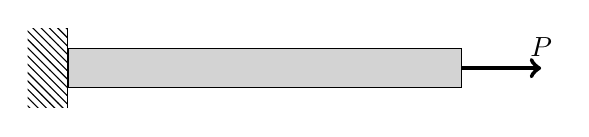
\begin{tikzpicture}
  \node[minimum height=1cm, minimum width=0.5cm, pattern=north west lines](wall){};
  \draw (wall.south east) -- (wall.north east);
  \node at (wall.east) [anchor=west, draw, minimum height=5mm, minimum width=5cm, fill=LightGrey](beam){};
  \draw [->, ultra thick] (beam.east) --++ (0:1) node[above]{$P$};
\end{tikzpicture}
\end{figure}
\end{itemize}
\end{frame}

\begin{frame}[label={sec:org933e5e4}]{Example: Same bars, Same forces, Different locations}
\begin{figure}[h]
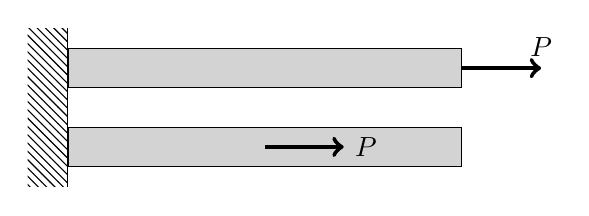
\begin{tikzpicture}
  \node[minimum height=2cm, minimum width=0.5cm, pattern=north west lines](wall){};
  \draw (wall.south east) -- (wall.north east);
  \node at (wall.east) [yshift=0.5cm, anchor=west, draw, minimum height=5mm, minimum width=5cm, fill=LightGrey](topbeam){};
  \node at (wall.east) [yshift=-0.5cm, anchor=west, draw, minimum height=5mm, minimum width=5cm, fill=LightGrey](bottombeam){};
  \draw [->, ultra thick] (topbeam.east) --++ (0:1) node[above]{$P$};
  \draw [->, ultra thick] (bottombeam.center) --++ (0:1) node[right]{$P$};
\end{tikzpicture}
\end{figure}
\end{frame}

\begin{frame}[label={sec:org9beaf11}]{Example: Deformation of a continuously variable bar}
\begin{itemize}
\item What is the elongation of the bar?

\begin{figure}[H]
  \centering
  % \includegraphics[scale=0.6]{pictures/Axial-load/axial-load-cone}
  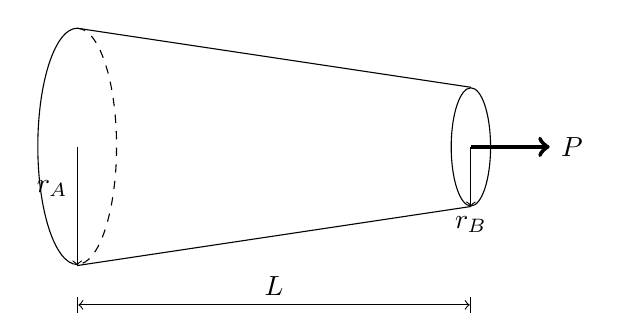
\begin{tikzpicture}
    \node [ellipse, dashed, minimum height=3cm, minimum width=1cm](left){};
    \draw (left.north) arc (90:270:0.5 and 1.5);
    \draw [dashed] (left.north) arc (90:-90:0.5 and 1.5);
    \node [ellipse, xshift=5cm, minimum height=1.5cm, minimum width=0.5cm, draw](right){};
    \draw
    (left.north) -- (right.north)
    (left.south) -- (right.south);
    \draw [->] (left.center) -- (left.south) node[midway, above left]{$r_A$};
    \draw [->] (right.center) -- (right.south) node[below]{$r_B$};
    \draw [->, ultra thick] (right.center) --++ (0:1) node[right]{$P$};
  \draw [|<->|] (left.south) ++ (-90:0.5) --++ (0:5) node[midway, above]{$L$};
  \end{tikzpicture}
\end{figure}
\end{itemize}
\end{frame}

\begin{frame}[label={sec:org054d555}]{Solution}
\begin{itemize}
\item load is constant throughout the length of the cylinder

\item area is not constant

\item we must use

\begin{align*}
  \delta  = \int_0^L d\delta  = \int_0^L \frac{Pdx}{EA(x)}
\end{align*}

\item need to write area as a function of length \(A = A(x)\)
\end{itemize}
\end{frame}

\begin{frame}[label={sec:org3a87405}]{Solution}
\begin{itemize}
\item Since the cylinder is actually a cone, radius \(r\) of area \(A\) is a linear function of \(x\)

\begin{align*}
  r = mx + c
\end{align*}

where \(m\) is the slope and \(c\) is the y-intercept

\item we know that at \(x = 0, r = r_{A}\) and at \(x = L, r = r_{B}\)

\begin{align*}
  m &= \frac{dr}{dx} = \frac{\Delta r}{\Delta x} = \frac{r_{B} - r_{A}}{L} \\
  c &= r(x = 0) = r_{A} \\
  r &=  \frac{r_{B} - r_{A}}{L} x + r_{A}
\end{align*}
\end{itemize}
\end{frame}

\begin{frame}[label={sec:orgf10161c}]{Solution}
\begin{itemize}
\item We can now evaluate the integral

\begin{align*}
  \delta &= \int_{0}^{L} \frac{Pdx}{E \pi \left( \dfrac{r_{B} - r_{A}}{L} x + r_{A} \right)^{2}} \\
         &= - \frac{PL}{\pi E \left( r_{B} - r_{A}  \right)} \left[ \frac{1}{ \dfrac{ r_{B} - r_{A} }{L} x + r_{A} } \right]_{0}^{L} \\
         &= - \frac{PL}{\pi E \left( r_{B} - r_{A}  \right)} \left[ \frac{1}{r_{B}} - \frac{1}{r_{A}} \right] \\
         &= \frac{PL}{\pi E r_{A} r_{B}}
\end{align*}
\end{itemize}
\end{frame}

\section{Statically Indeterminate Problems}
\label{statically-indeterminate-problems}
\begin{frame}[label={sec:orgcc6c9fd}]{Statically Indeterminate Axially Loaded Members}
\begin{itemize}
\item For statically determinate problems, equilibrium is sufficient

\item When members are constrained, equilibrium is not enough
\end{itemize}
\end{frame}

\begin{frame}[label={sec:org0ed21d0}]{Compatibility or Kinematic Conditions}
\begin{itemize}
\item Fortunately, constraints typically provide geometric conditions
\(\rightarrow\) compatibility equations

\item Constraints \(\rightarrow\) restriction of deformation
\end{itemize}
\end{frame}

\begin{frame}[label={sec:org9b5d3e6}]{Example: Basic Bar between Two Walls}
\begin{columns}
\begin{column}{0.5\columnwidth}
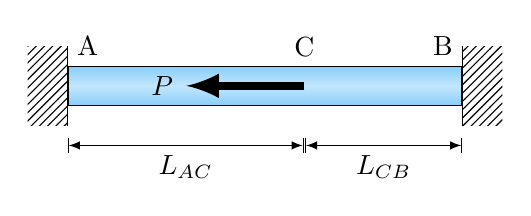
\begin{tikzpicture}[>=latex]
  \node [rectangle, pattern=north east lines, minimum height=1cm, minimum width=0.5cm](lwall){};
  \draw (lwall.south east) -- (lwall.north east);
  \node at (lwall.east) [anchor=west, draw, rectangle, top color=LightSkyBlue, bottom color=LightSkyBlue, middle color=LightSkyBlue!50, minimum height=5mm, minimum width=5cm](bar){};
  \node at (bar.east) [anchor=west, rectangle, pattern=north east lines, minimum height=1cm, minimum width=0.5cm](rwall){};
  \draw (rwall.south west) -- (rwall.north west);
  \node at (bar.north west) [above right]{A};
  \node at (bar.north east) [above left]{B};
  \draw [->, line width=3pt] (bar.center) ++ (0:0.5) node[above, yshift=0.2cm]{C} --++ (180:1.5) node[left]{$P$};
  \draw [|<->|] (bar.south west) ++ (-90:0.5) --++ (0:3) node[midway, below]{$L_{AC}$};
  \draw [|<->|] (bar.south east) ++ (-90:0.5) --++ (180:2) node[midway, below]{$L_{CB}$};
\end{tikzpicture}
\end{column}

\begin{column}{0.5\columnwidth}
\begin{itemize}
\item Equilibrium equation

$$ F_B + F_A - P = 0 $$

\item Compatibility equation: fixed between two walls = no deformation

\begin{gather*}
  \delta_{AB} = 0 \\
  \frac{F_A L_{AC}}{AE} - \frac{F_B L_{CB}}{AE} = 0 \\
  F_A = P \frac{L_{CB}}{L}; F_B = P \frac{L_{AC}}{L}
\end{gather*}
\end{itemize}
\end{column}
\end{columns}
\end{frame}

\begin{frame}[label={sec:org9946ab9}]{Solving SI Problems}
\begin{enumerate}
\item Draw FBD of member(s)

\item Write equilibrium equation(s)

\item Consider geometry restrictions or constrains

\item Express them in compatibility equations

\item Apply Hooke's law to compatibility equations and solve
\end{enumerate}
\end{frame}

\begin{frame}[label={sec:org86bcfc5}]{Example: Three Bars attached to Rigid Beam}
\begin{figure}[H]
  \centering
  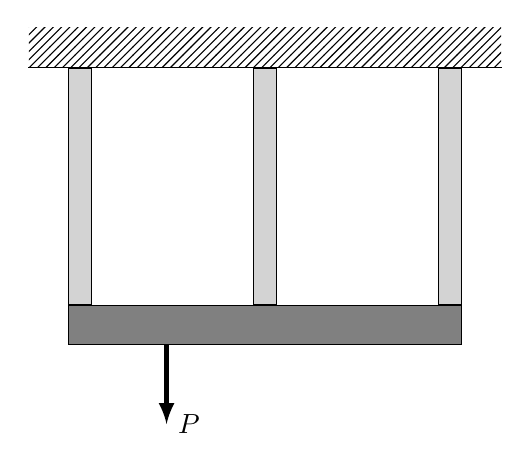
\begin{tikzpicture}[>=latex]
    \node [draw, rectangle, minimum height=0.5cm, minimum width=5cm, fill=Grey](rigid){};
    \node at (rigid.north west) [anchor=south west, draw, fill=LightGrey, minimum height=3cm, minimum width=3mm](left){};
    \node at (rigid.north) [anchor=south, draw, fill=LightGrey, minimum height=3cm, minimum width=3mm](mid){};
    \node at (rigid.north east) [anchor=south east, draw, fill=LightGrey, minimum height=3cm, minimum width=3mm](right){};
    \node at (mid.north) [anchor=south, minimum height=5mm, minimum width=6cm, pattern=north east lines](ceil){};
    \draw (ceil.south west) -- (ceil.south east);
    \draw [->, ultra thick] (rigid.south) ++ (180:1.25) --++ (-90:1) node[right]{$P$};
  \end{tikzpicture}
\end{figure}

\begin{itemize}
\item What are the forces in the bars if they have the same \(E\), \(A\)?
\end{itemize}
\end{frame}

\begin{frame}[label={sec:org2d5a9d1}]{Solution}
Assuming all internal forces are tensile, they all point upward on the
rigid beam.

Equilibrium:

\begin{gather*}
    \sum F_{y} = 0 \\
    F_1 + F_2 + F_3 = P
\end{gather*}

\begin{gather*}
    \sum M = 0 \\
    F_2 L + F_3 (2L) = P \frac{L}{2} \\
    F_2 + 2F_3 = \frac{P}{2}
\end{gather*}
\end{frame}

\begin{frame}[label={sec:org023fa0d}]{Solution}
Rigid beam can tilt, but not bend. Use similar triangles, compatibility equation is:

\begin{align*}
    \frac{\delta_1 - \delta_3}{2L} = \frac{\delta_2 - \delta_3}{L} \\
    \delta_1 - \delta_3 = 2\delta_2 - 2\delta_3 \\
    \delta_1 = 2\delta_2 - \delta_3
\end{align*}

Convert compatibility to force equation using Hooke's Law

\begin{gather*}
    \frac{F_1 L}{AE} = 2\frac{F_2 L}{AE} - \frac{F_3 L}{AE} \\
    F_1 = 2F_2 - F_3
    F_2 = \frac{P}{2} - 2F_3 \\
    F_1 = 2F_2 - F_3 = P - 5F_3
\end{gather*}
\end{frame}

\begin{frame}[label={sec:org882323e}]{Solve for the forces}
Now, substitute this into the first equilibrium equation.
\begin{align*}
   F_1 + F_2 + F_3 &= P - 5F_3 + \frac{P}{2} - 2F_3 + F_3 = P \\
   6F_3 &= \frac{P}{2} \\
   F_3 &= \frac{P}{12} \\
   F_1 &= P - 5 \frac{P}{12} = \frac{7P}{12} \\
   F_2 &= \frac{P}{2} - \frac{2P}{12} = \frac{P}{3}
\end{align*}
\end{frame}

\begin{frame}[label={sec:orgb7a8aa5}]{Thermal Strains: Oh It's Baaacccckkkk!!!!}
\begin{itemize}
\item Remember this?
\end{itemize}

\begin{align*}
  \frac{1}{L}\frac{dL}{dT} &= \alpha \\
  \varepsilon_T &= \alpha \Delta T = \alpha \left( T_2 - T_1 \right)
\end{align*}
\end{frame}

\begin{frame}[label={sec:org07f23dc}]{Temperature + Force = Pain}
\begin{itemize}
\item Thermal stress \(\rightarrow\) temperature change while constrained

\item Combination of mechanical and thermal loads

\item How do we deal with all dis shite?

\item Superposition! \(\rightarrow\) a fancy way of saying just add them up
\end{itemize}
\end{frame}

\begin{frame}[label={sec:org80a3b08}]{Example: Thermal Stress in Fastened Bars}
\begin{figure}[H]
  \centering
  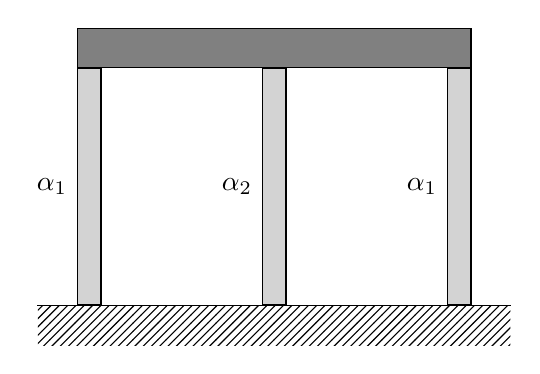
\begin{tikzpicture}[>=latex]
    \node [draw, rectangle, minimum height=0.5cm, minimum width=5cm, fill=Grey](rigid){};
    \node at (rigid.south west) [anchor=north west, draw, fill=LightGrey, minimum height=3cm, minimum width=3mm](left){};
    \node at (left.west) [left] {$\alpha_{1}$};
    \node at (rigid.south) [anchor=north, draw, fill=LightGrey, minimum height=3cm, minimum width=3mm](mid){};
    \node at (mid.west) [left] {$\alpha_{2}$};
    \node at (rigid.south east) [anchor=north east, draw, fill=LightGrey, minimum height=3cm, minimum width=3mm](right){};
    \node at (right.west) [left] {$\alpha_{1}$};
    \node at (mid.south) [anchor=north, minimum height=5mm, minimum width=6cm, pattern=north east lines](ceil){};
    \draw (ceil.north west) -- (ceil.north east);
  \end{tikzpicture}
\end{figure}

\begin{itemize}
\item What are the forces in each beam when the temperature is changed by \(\Delta T\)?
\end{itemize}
\end{frame}

\begin{frame}[label={sec:org1a0babe}]{Solution}
Equilibrium equations
\begin{gather*}
   \sum F_{y}  = 0 \\
   F_1 + F_2 + F_3 = 0
\end{gather*}

Using symmetry,
\begin{align*}
    F_1 &= F_3 \\
    F_2 &= 2F_3 = 2F_1
\end{align*}

Or using moment equilibrium
\begin{gather*}
    \sum M = 0 \\
    F_2 L + F_3 (2L) = 0 \\
    F_2 = -2F_3
\end{gather*}
\end{frame}

\begin{frame}[label={sec:org871e71c}]{Solution}
Moment equilibrium about the right side of the rigid beam gives the same equation.
\begin{align*}
  F_2 = -2F_1 = -2F_3
\end{align*}

With symmetry, all bars undergo identical deformation.

Compatibility:
\begin{align*}
  \delta_1 = \delta_2 = \delta_3
\end{align*}

Hooke's Law:
\begin{align*}
\frac{F_1 L}{AE} + \alpha_1 \Delta TL = \frac{F_2 L}{AE} + \alpha_2 \Delta TL
\end{align*}
\end{frame}

\begin{frame}[label={sec:org3c229a6}]{Solution}
Substituting \(F_1 = F_2 / 2\), we have
\begin{gather*}
F_2 = \frac{2}{3} \left( \alpha_1 - \alpha_2 \right) \Delta T A E \\
F_1 = F_3 = \frac{1}{3} \left( \alpha_2 - \alpha_1 \right) \Delta T A E
\end{gather*}
\end{frame}

\begin{frame}[label={sec:org0fd4909}]{Analysis}
\begin{itemize}
\item All forces assumed tensile, so if the sign comes out positive, the force \emph{is} tensile. It is compressive otherwise.

\item Consider \(\alpha_1 > \alpha_2\) and \(\Delta T > 0\)

$$ F_2 > 0 \text{ and } F_1, F_3 < 0 $$

\item When the members are heated the left and right members will try to expand more than the middle one due to their higher coefficients of thermal expansion \(\alpha_1\). However, because of the rigid beam restriction, the left and right members are squeezed down, while the middle part is pulled. Other situations can be analyzed with similar logic.
\end{itemize}
\end{frame}

\begin{frame}[label={sec:org6260b7c}]{Compatibility Equation}
\begin{itemize}
\item One member: wall or support limits deformation

\item More members: walls or attachment to rigid parts dictates deformation

\item Check symmetry
\end{itemize}
\end{frame}

\section{Compound Bars}
\label{compound-bars}
\begin{frame}[label={sec:org3225bbf}]{Analysis of a Compound Bar}
\begin{center}
\includegraphics[width=.9\linewidth]{pictures/compound-bar.jpg}
\end{center}

\begin{itemize}
\item Multiple members that share the same deformations

\item A special case of statically indeterminate problem
\end{itemize}
\end{frame}

\begin{frame}[label={sec:orgf7291eb}]{Force in Member of Compound Bar}
\begin{itemize}
\item For any member
\end{itemize}

\begin{align*}
  \delta = \delta_i = \frac{F_i L_i}{E_i A_i} \\
  F_i = \frac{\delta E_i A_i}{L_i}
\end{align*}

\begin{itemize}
\item Equilibrium equation

\begin{align*}
  W = \sum F_i = \sum \frac{\delta E_i A_i}{L_i}
\end{align*}
\end{itemize}
\end{frame}

\begin{frame}[label={sec:org0f9f398}]{Governing Equation of Compound Bars}
\begin{itemize}
\item Fraction of force in member \emph{i}
\end{itemize}

\begin{align*}
  \frac{F_i}{W} = \frac{\dfrac{E_i A_i}{L_i}}{\displaystyle\sum \dfrac{E_i A_i}{L_i}}
\end{align*}

\begin{itemize}
\item Modulus of the compound bar, if members have the same length
\end{itemize}

\begin{align*}
    W &= F_1 + F_2 + \ldots \\
    \sigma \left(A_1 + A_2 + \ldots \right) &= \sigma_1 A_1 + \sigma_2 A_2 + \ldots \\
    \frac{\sigma}{\varepsilon} \left(A_1 + A_2 + \ldots \right) &= \frac{\sigma_1}{\varepsilon}A_1 + \frac{\sigma_2}{\varepsilon}A_2 + \ldots \\
    E_c \left(A_1 + A_2 + \ldots \right) &= E_1 A_1 + E_2 A_2 + \ldots \\
    E_c &= \frac{\sum EA}{\sum A}
\end{align*}
\end{frame}

\begin{frame}[label={sec:org61f0e78}]{Example: Helping out a Friend}
\begin{columns}
\begin{column}{0.3\columnwidth}
\begin{center}
\includegraphics[height=0.7\textheight]{./pictures/2-guys-one-boulder.pdf}
\end{center}
\end{column}

\begin{column}{0.7\columnwidth}
\begin{itemize}
\item Two equal length and cross section cables: steel (\(E\) = 210 GPa) and
copper (\(E\) = 80 GPa)

\item Boulder weighs 200 kg

\item Who's carrying heavier load?
\end{itemize}
\end{column}
\end{columns}
\end{frame}

\section{Impact Loading}
\label{impact-loading}
\begin{frame}[label={sec:org73d552f}]{Object under Impact Loading}
\begin{figure}[h]
  \centering
  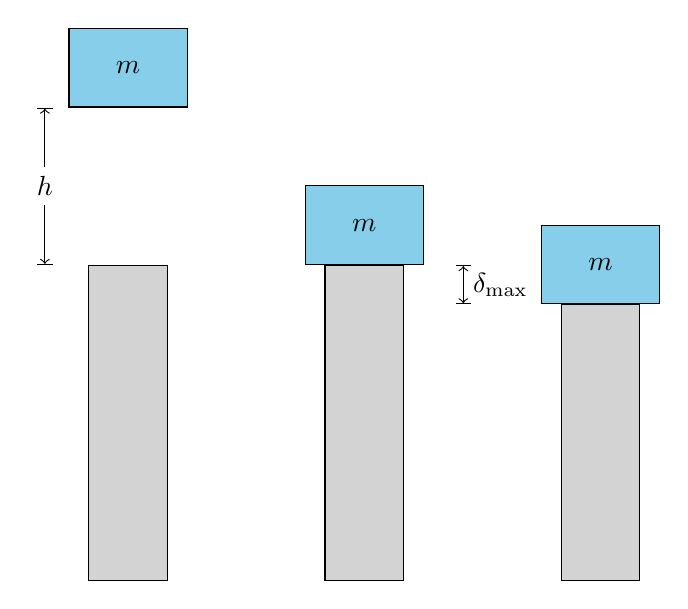
\begin{tikzpicture}
    \node [draw, rectangle, fill=LightGrey, minimum height=4cm, minimum width=1cm](lcol){};
    \node at (lcol.north)[anchor=south, yshift=2cm, draw, rectangle, fill=SkyBlue, minimum height=1cm, minimum width=1.5cm](lbox){$m$};
    \draw [|<->|] (lbox.south west) ++ (180:0.3) --++ (-90:2) node[midway, fill=white]{$h$};
    \node [xshift=3cm, draw, rectangle, fill=LightGrey, minimum height=4cm, minimum width=1cm](mcol){};
    \node at (mcol.north)[anchor=south, draw, rectangle, fill=SkyBlue, minimum height=1cm, minimum width=1.5cm](mbox){$m$};
    \node at (mcol.south) [anchor=south, xshift=3cm, draw, rectangle, fill=LightGrey, minimum height=3.5cm, minimum width=1cm](rcol){};
    \node at (rcol.north)[anchor=south, draw, rectangle, fill=SkyBlue, minimum height=1cm, minimum width=1.5cm](rbox){$m$};
    \draw [|<->|] (mbox.south east) ++ (0:0.5) --++ (-90:0.5) node[midway, right]{$\delta_{\max}$};
  \end{tikzpicture}
\end{figure}
\end{frame}

\begin{frame}[label={sec:orge623bbe}]{Maximum Deformation under Impact Loading}
\begin{itemize}
\item Weight dropped from \(h\)
\end{itemize}

\begin{gather*}
    W\left(h + \delta_{\max} \right) = \frac{EA\delta_{\max}^2}{2L} \\
    \delta_{\max} = \frac{WL}{EA} + \left[ \left( \frac{WL}{EA} \right)^2 + 2h \left( \frac{WL}{EA} \right) \right]^{1/2}
\end{gather*}

\begin{itemize}
\item But what is \(\dfrac{WL}{EA}\)?
\end{itemize}
\end{frame}

\begin{frame}[label={sec:org2215add}]{Max Deformation Compared to Static Load Deformation}
\begin{itemize}
\item Max deformation in terms of static deformation

\begin{gather*}
  \delta_{\max} = \delta_{st} + \left[ \delta_{st}^2 + 2h \delta_{st} \right]^{1/2}
\end{gather*}

\item When \(h \gg \delta_{st}\)
\begin{gather*}
  \delta_{\max} = \sqrt{2h \delta_{st}} = \sqrt{ \dfrac{mv^2 L}{EA} }
\end{gather*}
\end{itemize}
\end{frame}

\begin{frame}[label={sec:org7a0340a}]{Maximum Stress from Impact Loading}
\begin{itemize}
\item Since \(\delta = \dfrac{\sigma L}{E}\)
\end{itemize}

\begin{align*}
    \sigma_{\max} &= \frac{E\delta_{\max}}{L} \\
    \sigma_{\max} &= \frac{W}{A} + \left[ \left( \frac{W}{A} \right)^2 + \frac{2hE}{L}\frac{W}{A} \right]^{1/2} \\
    \sigma_{\max} &= \sigma_{st} + \left[ \left( \sigma_{st} \right)^2 + \frac{2hE}{L} \sigma_{st} \right]^{1/2}
\end{align*}

\begin{itemize}
\item If \(h\) is large

\begin{align*}
  \sigma_{\max} = \sqrt{ \frac{2hE}{L} \sigma_{st} } = \sqrt{ \frac{mv^2 E}{AL} }
\end{align*}
\end{itemize}
\end{frame}

\begin{frame}[label={sec:orge1bd175}]{Example: Drop Test}
Determine the maximum allowable mass \(m\) that you
can drop from the height \(h\) of 3 m a concrete block with \(A\) = 1
cm\(^{2}\), \(E\) = 80 GPa, and \(L\) = 0.5 m so that the the resultant
stress is below \(\sigma_{\text{allow}}\) = 10 MPa and
\(\delta_{\max} <\) 3 mm.
\end{frame}

\begin{frame}[label={sec:orgd48c47d}]{Solution}
2 conditions: \(\sigma_{\text{allow}}\) vs \(\delta_{\max}\)

\(\sigma_{\text{allow}}\):

\begin{align*}
    \sigma_{\text{allow}} &= \sigma_{\max} = \frac{W}{A} + \left[ \left( \frac{W}{A} \right)^{2} + \frac{2hE}{L}\frac{W}{A} \right]^{1/2} \\
    10 \times 10^{6} &= \frac{W}{1 \times 10^{-4}} + \left[ \left( \frac{W}{1 \times 10^{-4}} \right)^{2} + \frac{2(3)(80 \times 10^{9})}{0.5}\frac{W}{1 \times 10^{-4}} \right]^{1/2} \\
    W &= 0.01 \text{ N} \\
    m &= 0.01/10 = 0.001 \text{ kg}
\end{align*}
\end{frame}

\begin{frame}[label={sec:org821faf4}]{Solution}
We can also use the approximation (as a 3-m drop is pretty high, probably much higher than \(\delta_{st}\)). Instead,

\begin{align*}
    \sigma_{\max} &= \sqrt{\frac{2hE}{L} \sigma_{st}} \\
    10 \times 10^{6} &= \sqrt{\frac{2(3)(80 \times 10^{9})}{0.5}\sigma_{st}} \\
    \sigma_{st} &= 104 \\
    \frac{mg}{A} &= \frac{m(10)}{1 \times 10^{-4}} = 104 \\
    m &= 0.00104 \text{ kg}
\end{align*}

So we have essentially obtained the same answer.
\end{frame}

\begin{frame}[label={sec:orgdb0eebe}]{Solution \(\delta_{\max}\):}
\begin{align*}
    \delta_{\max} &= 0.003 = \frac{WL}{EA} + \left[ \left( \frac{WL}{EA} \right)^{2} + 2h \left( \frac{WL}{EA} \right) \right]^{1/2} \\
    0.003 &= \frac{W(0.5)}{80 \times 10^{9}(10^{-4})} + \left[ \left( \frac{W(0.5)}{80 \times 10^{9}(10^{-4})} \right)^{2} + 2h \left(  \frac{W(0.5)}{80 \times 10^{9}(10^{-4})} \right) \right]^{1/2} \\
    W &= 24 \text{ N} \\
    m &= 24/10 = 2.4 \text{ kg}
\end{align*}
\end{frame}

\begin{frame}[label={sec:org6338f4d}]{Solution}
Let's again try the short method and compare.

\begin{align*}
    \delta_{\max} &= \sqrt{2h\delta_{st}} \\
    0.003 &= \sqrt{2(3)\delta_{st}} \\
    \delta_{st} &= 1.5 \times 10^{-6} = \frac{WL}{EA} \\
    W = mg &= \frac{1.5 \times 10^{-6}(80 \times 10^{9})(1 \times 10^{4})}{0.5} = 24 \\
    m &= 24/10 = 2.4 \text{ kg}
\end{align*}

The smaller of the two l0ads, 0.001 kg is our final answer.
\end{frame}
\end{document}